%24/09 - Álvaro García
\chapter{Procesado imágenes digitales}
\section{Introducción}
El preprocesado y la mejora de imágenes tienen como objetivo:
\begin{itemize}
\item Realzar o mejorar el contraste.
\item Recortar (\textit{cropping}) o seleccionar regiones de interés.
\item Registrar: ajustar la geometría de una imagen para alinearla con otra.
\item Reducir o eliminar ruido y artefactos.
\item Corregir el desenfoque (\textit{deblurring}) o reconstruir áreas faltantes (\textit{inpainting}).
\end{itemize}

Un operador puntual se define de la siguiente manera:
Dada una imagen de entrada, el operador calcula cada píxel de la imagen de salida únicamente en función del valor del píxel en la misma posición (x, y) de la imagen de entrada, mediante una función matemática.

Un operador local, en cambio, calcula cada píxel de salida en función del píxel en la misma posición y de los píxeles de su vecindario en la imagen de entrada. La dependencia del vecindario está implícita en la función del operador.

\section{Operadores puntuales}
\subsection{Introducción}
Una transformación píxel a píxel donde el vecindario considerado es de 1x1, es decir, el propio píxel. Esto implica que las coordenadas espaciales del píxel son irrelevantes para la transformación. Se define como una transformación de los valores de intensidad de entrada, $r_k$, a valores de salida, $s_k$. Así, es un operador que modifica el nivel de gris de cada píxel individualmente. Estos operadores alteran la amplitud de los píxeles de acuerdo con una operación específica, lo que puede expandir la escala de grises para mejorar la visualización de detalles.

\begin{figure}[h]
\centering
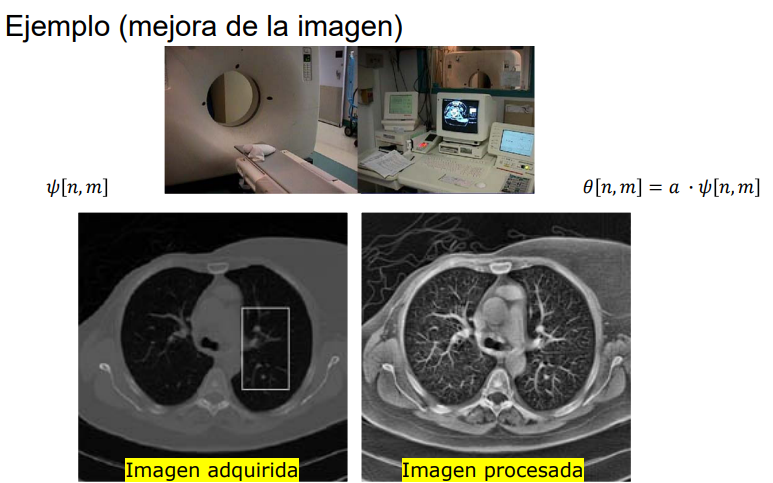
\includegraphics[width = 0.7\textwidth]{figs/mejora-puntual.png}
\end{figure}

\subsection{Modelado de histograma}
El histograma de una imagen $\psi[n,m]: h(r_k)$ denotado como $h(r_k)$, es una representación gráfica de la frecuencia de los niveles de gris. $h(r_k)$) indica el número de píxeles que tienen el valor $r_k$. 

Mientras la imagen original es bidimensional (coordenadas n, m), el histograma es unidimensional, ya que solo representa la distribución de frecuencias de los niveles de gris, sin información espacial.

\begin{figure}[h]
\centering
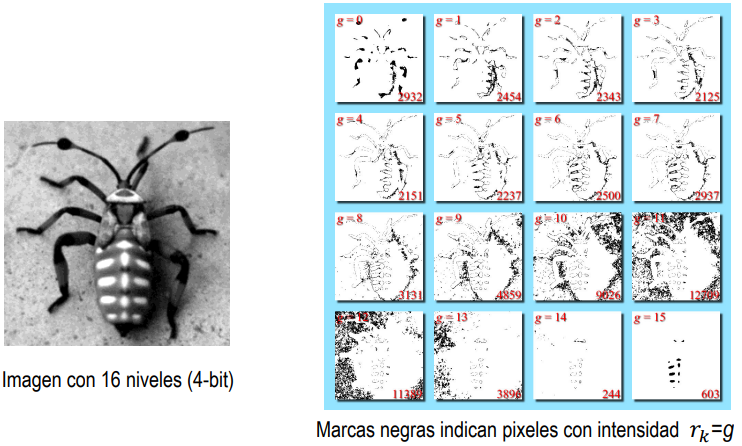
\includegraphics[width = 0.7\textwidth]{figs/histograma1.png}
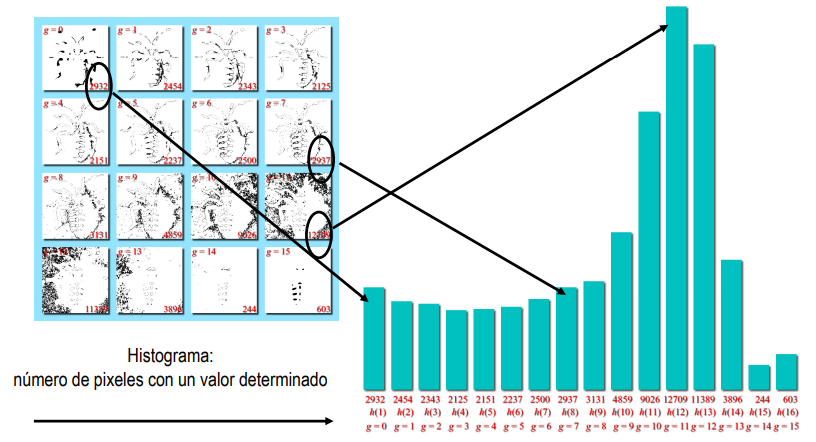
\includegraphics[width = 0.7\textwidth]{figs/histograma2.png}
\end{figure}

El histograma normalizado, obtenido al dividir cada valor del histograma por el número total de píxeles (ancho x alto de la imagen), estima la \textbf{función de densidad de probabilidad (FDP)} de los niveles de gris. La suma de todos sus valores es 1. Al acumular estos valores, se obtiene la \textbf{función de distribución acumulativa (FDA)} de la imagen, que siempre culmina en 1.

\begin{figure}[h]
\centering
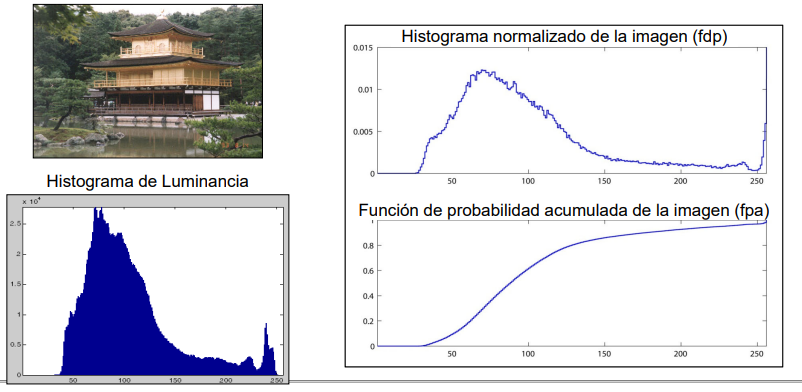
\includegraphics[width = 0.7\textwidth]{figs/fdp-fpa.png}
\end{figure}

Una limitación importante del histograma es que \textbf{no contiene información espacial} sobre la disposición de los píxeles en la imagen.

\subsubsection{Ajuste de contraste}
El objetivo es realzar imágenes con bajo contraste, causado por condiciones de baja iluminación, un rango dinámico limitado del sensor o errores en la configuración de la cámara (como la apertura del diafragma). La solución consiste en expandir o comprimir el rango dinámico de las intensidades según sea necesario.

Para expandir el contraste, se asigna un rango más amplio de valores de salida a un rango estrecho de valores de entrada en el histograma. Para reducir el contraste, se hace lo contrario. El objetivo es aprovechar todo el rango disponible de niveles de gris.

\begin{figure}[h]
\centering
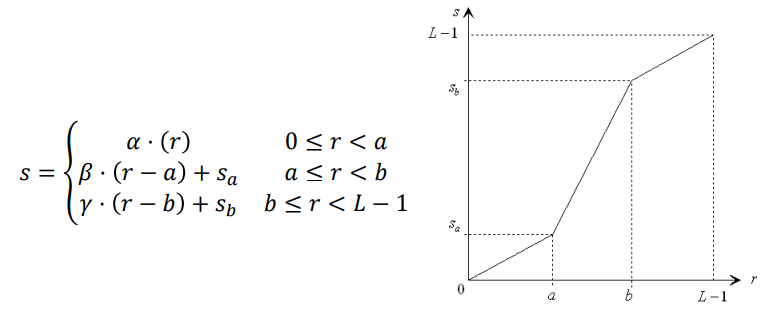
\includegraphics[width = 0.7\textwidth]{figs/ajuste-contraste.png}
\end{figure}

\begin{figure}[h]
\centering
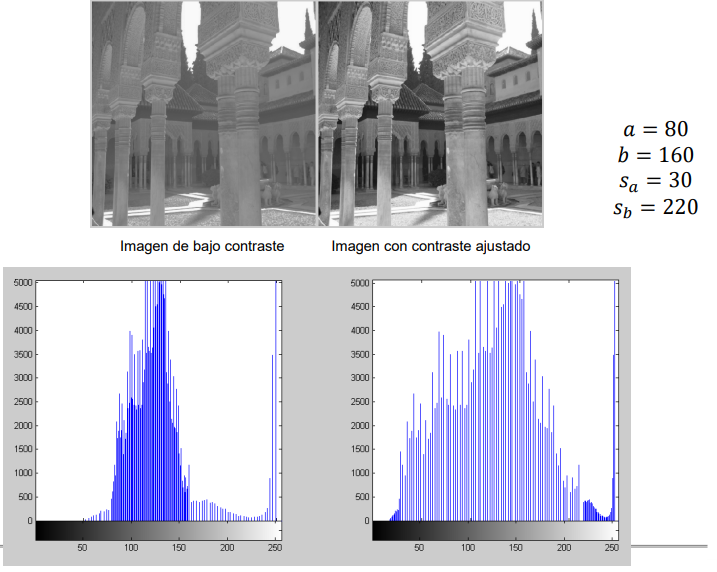
\includegraphics[width = 0.6\textwidth]{figs/ajuste-contraste-ej.png}
\end{figure}

En el ejemplo, un valor de entrada de 80 se transforma en 30, y un valor de 160 en 220. Esto expande el rango central de intensidades y comprime los extremos, logrando una mejor distribución del contraste.

\subsubsection{Igualación o ecualización (\textit{equalization)}}
La ecualización busca que la imagen resultante tenga un histograma lo más uniforme posible, es decir, que todos los niveles de gris tengan una frecuencia similar. Para ello, se utiliza la función de distribución acumulativa (FDA) del histograma normalizado como función de transformación. El efecto es una mejora continua y automática del contraste, a diferencia del ajuste por tramos.

\begin{figure}[h]
\centering
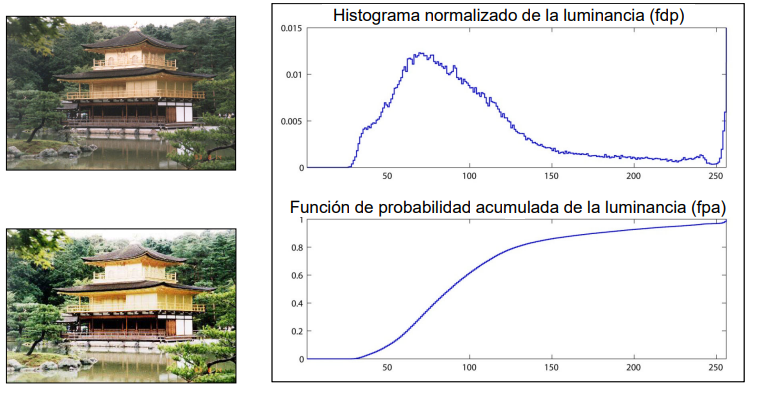
\includegraphics[width = 0.6\textwidth]{figs/equalization1.png}
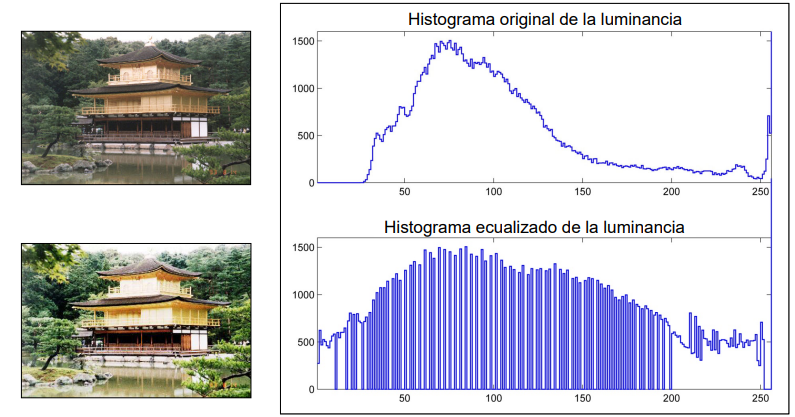
\includegraphics[width = 0.6\textwidth]{figs/equalization.png}
\end{figure}

La nueva intensidad de un píxel se calcula aplicando su FDA al rango máximo de grises (ej., 255). Por ejemplo, si la FDA de un nivel de gris es 0.6, su nuevo valor será $0.6 \cdot 255 \approx 153$.

\subsection{Modificación de niveles}
Estas técnicas permiten seleccionar información específica o crear efectos especiales modificando el histograma indirectamente. Los tipos principales son:
\begin{itemize}
\item \textbf{Recorte (\textit{clipping}):}

Similar al ajuste de contraste, pero "recorta" los valores por encima y por debajo de unos umbrales, asignándoles el valor máximo o mínimo. Las pendientes fuera del rango de interés se vuelven cero. Es útil para aislar regiones de interés o eliminar ruido cuando se conoce el rango válido de intensidades.

\begin{figure}[h]
\centering
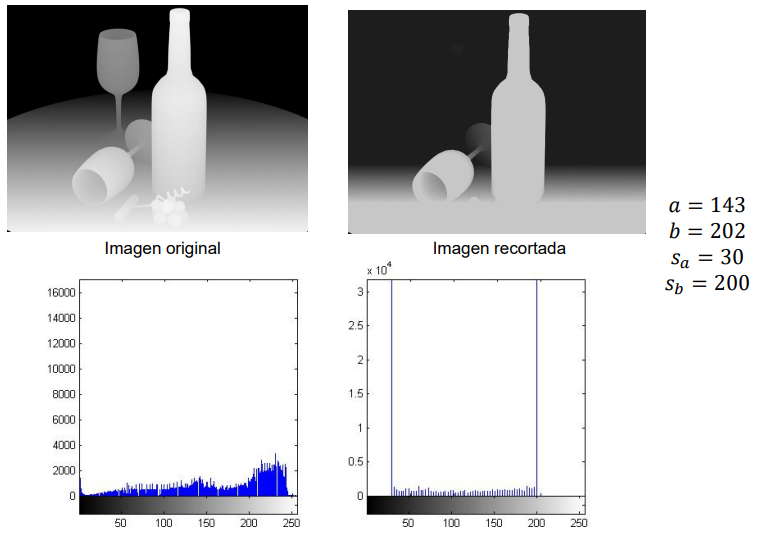
\includegraphics[width = 0.6\textwidth]{figs/recorte.png}
\end{figure}

Se utiliza, por ejemplo, en sistemas de ayuda a la conducción para ignorar obstáculos lejanos, o en robótica para limitar la percepción a distancias relevantes.

\item \textbf{Negativo o Inversión del eje de intensidades}:

Invierte los valores de intensidad (el blanco se vuelve negro y viceversa). Es útil en el análisis de imágenes médicas, como radiografías, para cambiar la perspectiva visual. El histograma resultante es la imagen especular del original.

\item \textbf{Seccionado de niveles (\textit{slicing}):}

Busca aislar una banda específica de niveles de gris, ya sea para extraerla o para resaltarla sobre el fondo.

\begin{figure}[h]
\centering
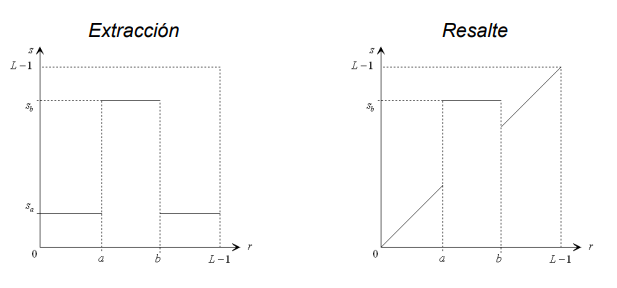
\includegraphics[width = 0.7\textwidth]{figs/extraccion-resalte.png}
\end{figure}

\begin{figure}[h]
\centering
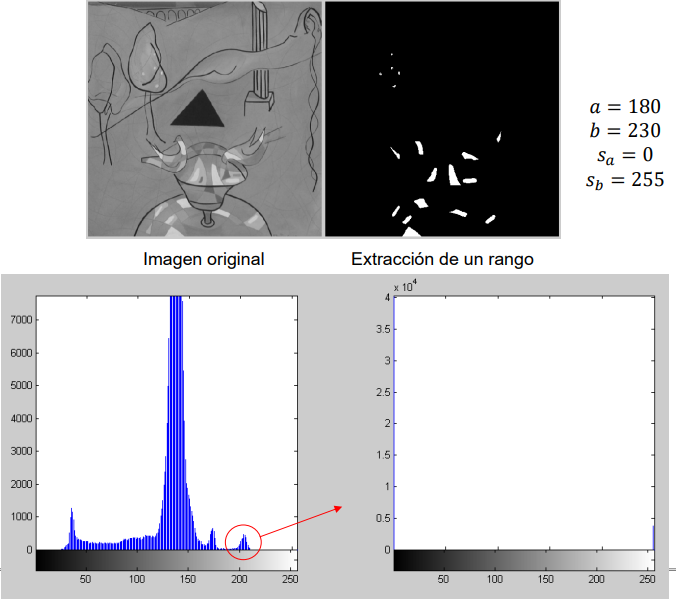
\includegraphics[width = 0.5\textwidth]{figs/extraccion-ej.png}
\caption{Ejemplo de extracción. Los píxeles dentro del rango seleccionado se muestran en blanco; el resto en negro.}
\end{figure}

\begin{figure}[h]
\centering
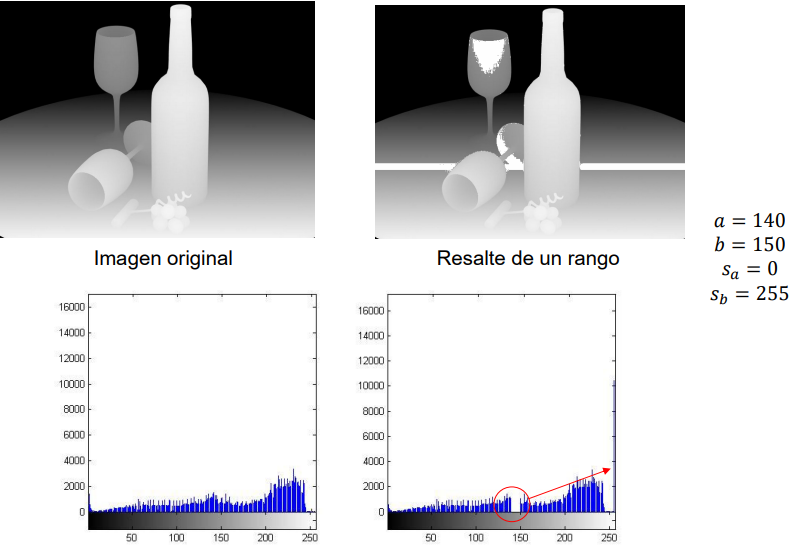
\includegraphics[width = 0.5\textwidth]{figs/resalte-ej.png}
\caption{Ejemplo de resalte. Una banda específica (ej., 140-150) se resalta en blanco. Puede usarse en sistemas de asistencia al conductor para marcar los límites de la distancia de seguridad.}
\end{figure} 
\end{itemize}

\section{Operadores locales}
Los operadores locales efectúan una transformación en el dominio espacial, conocida como \textit{filtrado espacial}.

\subsection{Filtrado espacial}
La operación de convolución se expresa como:
$$\theta [n,m] = \psi [n,m] \ast h[n,m] = \sum^a_{k=-1} \sum^b_{l=-b} \psi[k,l] \cdot h[n-k,m-l]$$

Para calcular $\theta[n,m]$, se centra la máscara invertida $h[-n,-m]$ sobre el píxel $\psi[n,m]$ y se calcula la suma de los productos de los píxeles de la vecindad por los coeficientes correspondientes de la máscara.

\begin{figure}[h]
\centering
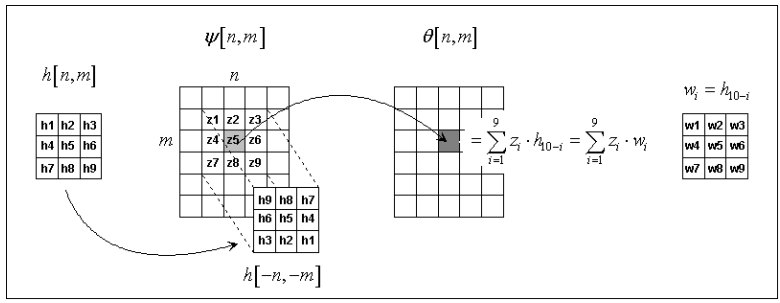
\includegraphics[width = 0.8\textwidth]{figs/convolution.png}
\end{figure}

La convolución de una imagen con un impulso (delta) desplaza la imagen. Por ejemplo, una máscara con un único '1' en una esquina desplazará la imagen. Si la máscara contiene varios impulsos, el resultado es una superposición de imágenes desplazadas y promediadas, lo que genera un efecto de emborronamiento.


Si en lugar de guardar solo 1 píxel de la matriz guardamos tres impulsos, se produce un desplazamiento y superposición. Se deben dividir entre 3 por normalización, y se guardan el píxel central, el píxel arriba a la izquierda y el píxel abajo a la derecha. Como se promedia, el resultado es una imagen movida emborronada.

Ahora guardamos 5 valores, las 4 esquinas y el valor central. La imagen resultante sigue estando movida. Esto se debe a que usualmente el vecindario no es tan grande. Si en lugar de utilizar un vecindario 16x16 se utiliza un vecindario 3x3, la convolución se convierte en un filtro de emborronado o suavizado que a simple vista no se aprecia, pero con zoom sí se aprecia que los bordes son más suaves al estar promediados.

En la práctica, se utilizan máscaras pequeñas (ej., 3x3). La convolución con una máscara de promediado produce un suavizado o desenfoque, haciendo los bordes menos nítidos.

Un desafío al aplicar convoluciones es el tratamiento de los bordes, donde la máscara se extiende más allá de la imagen. Las estrategias comunes para manejar esto son:
\begin{itemize}
\item \textbf{Relleno de ceros (\textit{Zero padding}):} Los píxeles fuera de la imagen se consideran 0.
\item \textbf{Réplica de píxeles (\textit{Replication}):} Se replican los valores de los píxeles del borde. Esta opción suele preferirse en imágenes médicas.
\item \textbf{Convolución circular:} La imagen se trata como periódica, tomando píxeles del lado opuesto.
\end{itemize}

\subsection{Suavizado: lineal y no lineal}
Los filtros de suavizado se utilizan para reducir ruido o difuminar detalles. En los filtros lineales, los coeficientes de la máscara son positivos y suman 1 para mantener el nivel de brillo promedio.

Los diseños comunes incluyen:
\begin{itemize}
\item \textbf{Filtro de media (\textit{averaging}):} Todos los coeficientes de la máscara son iguales.
\item \textbf{Filtro de media ponderada (\textit{weighted average}):} Los coeficientes son mayores en el centro, dando más peso al píxel central y a sus vecinos más cercanos. Un caso particular es el filtro binomial, que es separable y produce un suavizado más gradual.
\end{itemize}

La máscara de filtrado promediado ponderada es un caso particular de filtro binomial, familia de filtros separables resultante de la aplicación sucesiva y en ambas dimensiones de la máscara. El promediado da un resultado más borroso que el binomial.

El filtrado no lineal no se basa en una suma ponderada. Preserva mejor los bordes y es efectivo contra ruido impulsivo (como ruido sal y pimienta). Un caso paradigmático es el filtro de mediana, que reemplaza el valor del píxel central por la mediana de los valores en su vecindario. Otros filtros de estadísticas de orden son el de mínimo y el de máximo.

Filtro de mediana: en lugar de mezclar por igual, se aplica la función de la mediana. Se define un píxel central y un vecindario, y al vecindario se aplica la mediana. Eso mismo se puede hacer con el valor mínimo (filtro de mínimo), máximo (filtro de máximo) y filtro de posición. El filtro de mediana funciona muy bien para el ruido de sal-pimienta (puntos blancos y negros aleatorios). 

\begin{figure}[h]
\centering
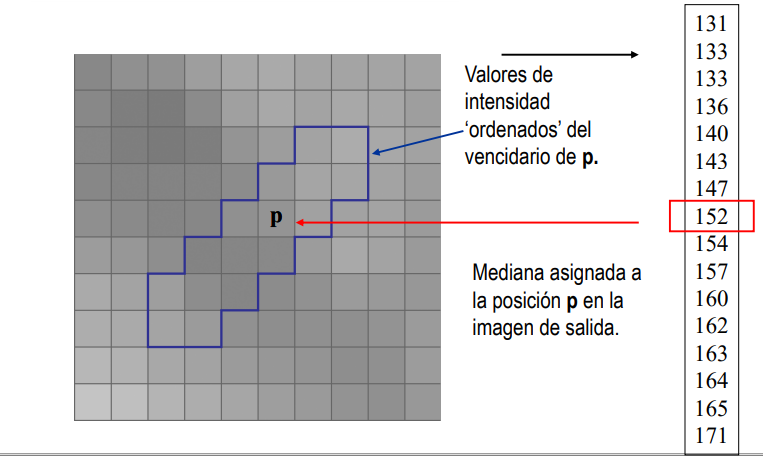
\includegraphics[width = 0.6\textwidth]{figs/filtro-median.png}
\end{figure}

\begin{figure}[h]
\centering
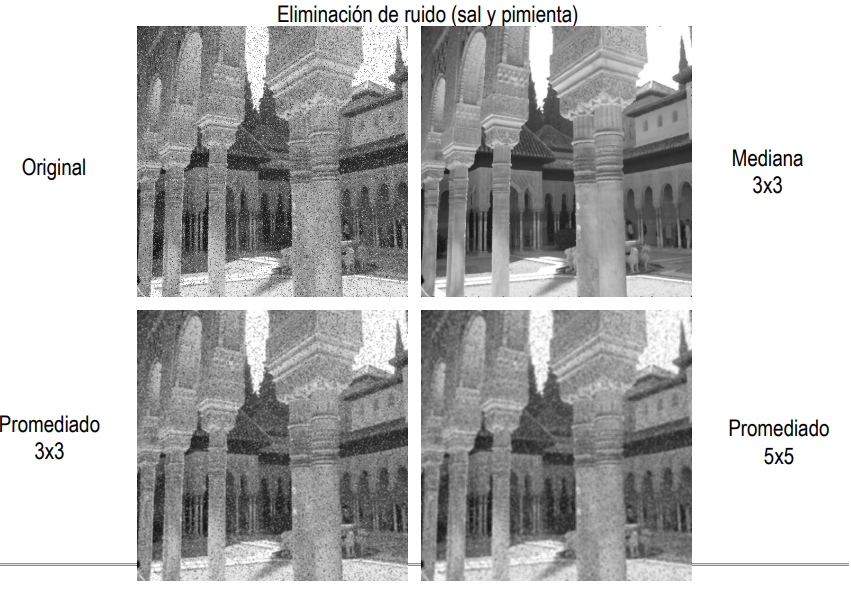
\includegraphics[width = 0.6\textwidth]{figs/sal-pimienta.png}
\end{figure}

\subsection{Realce: lineal}
Los filtros de realce resaltan detalles finos y bordes. Mientras el suavizado se asocia con la integración (promediado), el realce se relaciona con la derivación, que responde fuertemente a las discontinuidades (bordes) y al ruido.

En imágenes discretas, las derivadas se aproximan mediante diferencias. La primera derivada se implementa típicamente calculando la magnitud del gradiente. Los operadores más comunes para esto en máscaras 3x3 son los operadores de Prewitt, Sobel y Roberts.

El \textbf{operador de Prewitt} es un filtro de derivada parcial utilizado para calcular una aproximación del gradiente de la imagen en cada punto, lo que permite resaltar los bordes. Se compone de dos máscaras o kernels 3x3: una para calcular la derivada en la dirección horizontal (Gx) y otra para la dirección vertical (Gy).

\begin{figure}[h]
\centering
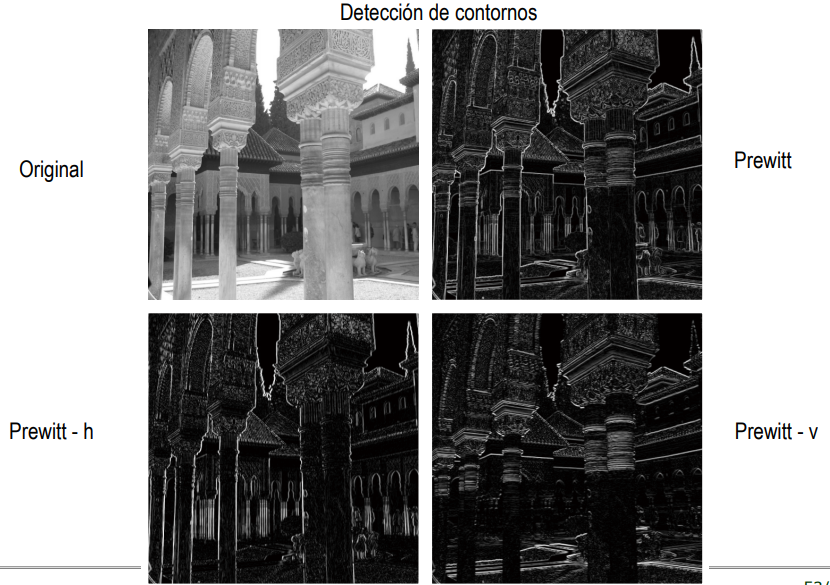
\includegraphics[width = 0.6\textwidth]{figs/prewitt.png}
\end{figure}